\documentclass[12pt]{article}

\usepackage[utf8]{inputenc}
\usepackage[T1]{fontenc}
\usepackage{graphicx}
\usepackage{amsmath}
\usepackage{amssymb}
\usepackage{fancyhdr}
\usepackage{geometry}
\usepackage{hyperref}
\usepackage{booktabs}
\usepackage{caption}
\usepackage{titlesec}

\geometry{margin=1in}

\hypersetup{
    colorlinks=true,
    linkcolor=black,
    citecolor=black,
    urlcolor=black
}

\newcommand{\shorttitle}{Reproducing SCI: Graph Embedding for Sub-Compartments}

\pagestyle{fancy}
\fancyhf{}
\renewcommand{\headrulewidth}{0pt}
\renewcommand{\footrulewidth}{0.4pt}
\fancyfoot[L]{\shorttitle}
\fancyfoot[R]{Page \thepage}

\titleformat{\section}{\large\bfseries}{\thesection.}{0.6em}{}
\titleformat{\subsection}{\normalsize\bfseries}{\thesubsection.}{0.6em}{}
\titleformat{\subsubsection}{\normalsize\bfseries}{\thesubsubsection.}{0.6em}{}

\newcommand{\sectionbreak}{\clearpage}

\begin{document}

% ---------------------------------------------------------------
% TITLE PAGE
% ---------------------------------------------------------------
\begin{titlepage}
\centering
\vspace*{1cm}
{\large\bfseries Mid-Sem Lab Project Report:}\\[0.8cm]
{\Large\bfseries Reproducing Sub-Compartment Identifier (SCI):\\
Graph Embedding Approaches for Genomic\\
Sub-Compartment Prediction from Hi-C Data}\\[1.5cm]

\includegraphics[width=4cm]{bits_logo.png}\\[1.5cm]

{\bfseries\large Harshal Shah}\\
(2023A7PS0055H)\\[1.5cm]

{\bfseries Under Guidance of}\\
{\bfseries\large Prof. Apurba Das}\\
(BITS Pilani, Hyderabad Campus)\\[1.5cm]

{Course Number: CS F367}
\vfill
\end{titlepage}

% ---------------------------------------------------------------
% CONTENTS
% ---------------------------------------------------------------
\tableofcontents
\clearpage

% ---------------------------------------------------------------
% ACKNOWLEDGMENTS
% ---------------------------------------------------------------
\section*{ACKNOWLEDGMENTS}
\addcontentsline{toc}{section}{ACKNOWLEDGMENTS}

I would like to express my sincere gratitude to my project guide, Prof. Apurba Das, for the
guidance and encouragement extended throughout the design and execution of this project.
His inputs on graph-based representation learning and genomic data analysis were instrumental
in shaping the direction of this work.

I would also like to thank the Birla Institute of Technology and Science (BITS), Pilani, Hyderabad
Campus, for providing the academic environment and computational resources necessary to carry
out this reproduction and comparative study.

Finally, I am grateful to my peers in the CS F367 course for the discussions on graph embedding
techniques and clustering evaluation that helped refine the comparative framework used in this
report, and to the maintainers of the open-source SCI and sci-DNN codebases, as well as the
developers of the scikit-learn, NumPy, and SciPy libraries, for making their implementations
publicly available and enabling this reproduction to be carried out without having to re-derive
these tools from first principles.

This work would also not have been possible without the computational infrastructure made
available for this course, which was essential for handling the genome-scale Hi-C graphs,
multi-hundred-megabyte interaction files, and dense similarity-matrix computations involved
in both the SCI reproduction and the HOPE-based extension.

Lastly, I acknowledge the original authors of the SCI methodology, Ashoor et al., whose
published work on graph embedding and unsupervised learning for genomic sub-compartment
prediction forms the foundation upon which both the reproduction and the HOPE-based extension
presented in this report are built.

% ---------------------------------------------------------------
% ABSTRACT
% ---------------------------------------------------------------
\section*{ABSTRACT}
\addcontentsline{toc}{section}{ABSTRACT}

The three-dimensional organization of the human genome inside the nucleus plays a central role
in regulating gene expression, and Hi-C chromatin conformation capture data has made it possible
to study this organization at genome-wide scale. Beyond the well-known A/B compartments, the
genome can be further partitioned into finer-grained \textit{sub-compartments} that carry distinct
epigenetic and transcriptional signatures. Sub-Compartment Identifier (SCI), proposed by
Ashoor et al. (2020), predicts these sub-compartments by embedding the Hi-C contact graph using
the LINE algorithm and clustering the resulting vectors with K-means.

This project reproduces the SCI pipeline end-to-end on the GM12878 cell line Hi-C dataset,
reconstructing the contact graph, generating LINE order-1 and order-2 embeddings, and clustering
them into five compartments. As an extension, an alternative graph embedding method, HOPE
(Higher-Order Proximity preserved Embedding), based on Katz-proximity and truncated Singular
Value Decomposition, was implemented and evaluated under the same clustering and evaluation
protocol. Both embeddings were scored using internal clustering-quality metrics (Silhouette Score,
Davies-Bouldin Index) and external agreement metrics against the SCI reference sub-compartment
calls (Adjusted Rand Index, Normalized Mutual Information). On this reproduction, the HOPE
embedding achieved an Adjusted Rand Index of 0.342 and a Normalized Mutual Information of
0.370 against the SCI reference labels, substantially higher than the reproduced LINE embedding's
0.00003 and 0.00017 respectively, indicating that order-1 Katz proximity recovers the genome's
sub-compartment structure considerably more effectively than this reproduction of LINE on the
same data. This report documents the reproduction methodology, the HOPE-based extension,
the evaluation framework, and the practical challenges encountered while working with
genome-scale Hi-C graphs.

The remainder of the report is organized as follows. Section~1 introduces the biological and
computational background of genomic sub-compartment prediction. Section~2 states the aims and
scope of this mid-term phase. Section~3 reviews the SCI, LINE, and HOPE literature that motivates
the methodology. Section~4 characterizes the GM12878 Hi-C dataset and the graph-construction
and SCI-reproduction procedure. Section~5 details the proposed HOPE-based methodology.
Sections~6 and 7 present the comparative results and the practical engineering challenges
encountered, respectively. Sections~8 and 9 close with planned future work and concluding
remarks, followed by a supporting appendix and the full reference list.

\clearpage

% ---------------------------------------------------------------
% 1. INTRODUCTION
% ---------------------------------------------------------------
\section{Introduction to Genome Sub-Compartment Prediction}

\subsection{Three-Dimensional Genome Organization and Hi-C}
Inside the nucleus, chromosomes are not arranged randomly; they fold into a hierarchy of structures
that brings distant genomic regions into physical proximity and influences how genes are
regulated. High-throughput Chromosome Conformation Capture (Hi-C) is a sequencing-based
technique that measures the frequency with which pairs of genomic loci come into contact,
producing a genome-wide contact matrix. At coarse resolution, principal component analysis of
this matrix reveals two large-scale compartments, conventionally labelled A (open, transcriptionally
active chromatin) and B (closed, transcriptionally repressed chromatin).

\subsection{Genomic Sub-Compartments}
Subsequent work using deeper Hi-C sequencing (Rao et al., 2014) showed that the simple A/B
division is itself a coarse summary of a finer structure: the genome can be partitioned into five
or more sub-compartments (commonly labelled A1, A2, B1, B2, B3) that differ in replication
timing, histone modification patterns, and transcription factor occupancy. Identifying these
sub-compartments accurately from Hi-C data, rather than from expensive orthogonal assays, is
the computational problem this project is concerned with.

\subsection{Graph-Based Sub-Compartment Calling}
A Hi-C contact matrix is naturally a weighted graph: genomic bins are nodes, and normalized
contact frequencies are edge weights. Sub-Compartment Identifier (SCI) treats sub-compartment
calling as a graph representation learning problem — it first embeds this contact graph into a
low-dimensional vector space using the LINE algorithm, so that bins with similar interaction
neighborhoods land close together, and then applies K-means clustering on the embeddings to
assign each bin to a sub-compartment. This project reproduces that pipeline and evaluates an
alternative embedding method, HOPE, as a point of comparison.


% ---------------------------------------------------------------
% 2. AIMS AND SCOPE
% ---------------------------------------------------------------
\section{Aims and Scope}

This mid-term phase of the project is scoped around reproducing a single, well-defined
published result — the SCI graph-embedding pipeline for genomic sub-compartment prediction —
and then extending it with one controlled architectural change: swapping the LINE embedding
for HOPE while holding the Hi-C graph, the clustering procedure, and the evaluation protocol
fixed. This design keeps the comparison between LINE and HOPE attributable to the embedding
method itself rather than to incidental differences in data processing or evaluation. The
objectives of this mid-term phase of the project are:

\begin{enumerate}
    \item \textbf{Reproduce the SCI Pipeline:} Clone and run the original SCI codebase on the
    GM12878 Hi-C dataset to generate reference sub-compartment predictions, following the
    graph-construction, LINE-embedding, and K-means-clustering procedure described by
    Ashoor et al. (2020).

    \item \textbf{Reproduce the Companion Classifier:} Set up and run sci-DNN, the deep neural
    network companion to SCI that predicts sub-compartments from epigenomic and
    sequence-derived features, to understand the full scope of the original work.

    \item \textbf{Implement an Alternative Graph Embedding:} Implement HOPE (Higher-Order
    Proximity preserved Embedding) using Katz-proximity similarity and truncated SVD as an
    alternative to LINE for embedding the same Hi-C contact graph.

    \item \textbf{Comparative Evaluation:} Cluster the HOPE embedding with the same K-means
    configuration used for the LINE reproduction, and evaluate both embeddings against the SCI
    reference sub-compartment calls using internal (Silhouette, Davies-Bouldin) and external
    (Adjusted Rand Index, Normalized Mutual Information) metrics.

    \item \textbf{Document Practical Challenges:} Record the engineering difficulties encountered
    while scaling graph-embedding computations to a genome-wide Hi-C graph with tens of
    thousands of nodes, and the solutions adopted.
\end{enumerate}

\textbf{Out of scope for this mid-term phase:} hyperparameter tuning of LINE beyond the SCI
reference configuration, inclusion of higher-order ($\beta^2 A^2$ and beyond) Katz terms in the
HOPE similarity matrix, validation against orthogonal ChIA-PET interaction data as performed in
the original SCI paper, and extension of the comparison to Hi-C datasets from cell lines other
than GM12878. These directions are deferred to the remainder of the project and are discussed
further in Section~8.


% ---------------------------------------------------------------
% 3. LITERATURE REVIEW
% ---------------------------------------------------------------
\section{Literature Review and Knowledge Acquisition}

\subsection{SCI: Graph Embedding and Unsupervised Learning for Sub-Compartments}
The primary reference for this project is Ashoor et al. (2020), \textit{``Graph embedding and
unsupervised learning predict genomic sub-compartments from HiC chromatin interaction data''},
published in \textit{Nature Communications}. The authors represent the Hi-C contact matrix as a
weighted graph and embed it using LINE (Large-scale Information Network Embedding), which
preserves both first-order proximity (direct contact strength between two bins) and second-order
proximity (similarity of two bins' contact neighborhoods). The resulting embeddings are clustered
with K-means to assign sub-compartment labels.

\textbf{Key Takeaways:} The authors show that SCI's topological-embedding approach outperforms
Hidden Markov Model (HMM)-based sub-compartment callers and that its predictions are
independently validated using orthogonal ChIA-PET interaction data. They further show that a
deep neural network (sci-DNN), trained using SCI-derived labels, can predict sub-compartments
directly from epigenomic, replication-timing, and sequence features, without needing a new Hi-C
experiment. This paper forms the methodological backbone reproduced in this project.

\subsection{Graph Embedding Methods: LINE versus HOPE}
To contextualize the choice of an alternative embedding method, two foundational graph embedding
papers were reviewed.

\textbf{LINE} (Tang et al., 2015) optimizes node embeddings by directly preserving first-order
proximity (observed edge weights) and second-order proximity (similarity of neighborhood
distributions) through stochastic gradient descent on a sampled edge set. It scales well to
large graphs but, being based on local neighborhood sampling, can be comparatively less sensitive
to longer-range, higher-order structure in the graph.

\textbf{HOPE} (Ou et al., 2016), \textit{``Asymmetric Transitivity Preserving Graph Embedding''},
instead preserves higher-order proximity measures (such as Katz index, Rooted PageRank, or
Common Neighbors) by factorizing a similarity matrix derived from the graph using a generalized
Singular Value Decomposition. Because Katz proximity aggregates information over paths of all
lengths (weighted by a decay factor $\beta$), HOPE embeddings can capture more global structural
relationships between nodes than embeddings built purely from local sampling.

This project implements HOPE with an order-1 Katz similarity (described in Section 5) as a
direct, like-for-like alternative to the LINE embedding used in the SCI reproduction, under an
identical downstream clustering and evaluation protocol.


% ---------------------------------------------------------------
% 4. DATASET AND PREPROCESSING
% ---------------------------------------------------------------
\section{Dataset Characterization and Preprocessing}

\subsection{GM12878 Hi-C Dataset}
The Hi-C dataset used throughout this project is derived from the GM12878 lymphoblastoid cell
line, provided in a bedpe-like format where each row records two interacting genomic bins
(chromosome, start, end for each bin) along with the corresponding Hi-C contact count. The raw
interaction file (\texttt{data/demo\_data.txt}) is approximately 513 MB, reflecting the scale of a
genome-wide Hi-C experiment.

\subsection{Hi-C Graph Construction}
The pairwise bin interactions were converted into a sparse, genome-wide adjacency matrix
(\texttt{results/repro\_test\_HiC\_graph.txt}) spanning 26,977 genomic bins, with each entry
representing the normalized contact weight between two bins. This adjacency structure is the
common input consumed by both the LINE and HOPE embedding stages described later in this
report.

\subsection{Reproducing the SCI Reference Pipeline}
The original SCI codebase was cloned and run on this adjacency graph, following its LINE-based
embedding procedure:

\begin{enumerate}
    \item \textbf{Order-1 and order-2 LINE embeddings} were trained separately on the Hi-C graph,
    each producing a 100-dimensional vector per bin that preserves either direct contact
    strength (order-1) or shared-neighborhood similarity (order-2).
    \item The two embeddings were \textbf{concatenated} into a single 200-dimensional vector per
    bin and \textbf{L2-normalized}, matching the procedure in SCI's own compartment-calling
    script.
    \item \textbf{K-means clustering} with $k=5$ was applied to the normalized, concatenated
    embedding to assign each bin one of five sub-compartment labels, producing
    \texttt{results/\allowbreak repro\_test\_compartments.txt}.
\end{enumerate}

In parallel, the reference sub-compartment calls published with the SCI repository for GM12878
(\texttt{repos/sci/predictions/\allowbreak GM12878\_SCI\_sub\_compartments.bed}) were retained
as the ground truth against which every subsequent embedding (including this project's own LINE
reproduction) is externally evaluated.


% ---------------------------------------------------------------
% 5. METHODOLOGY: HOPE
% ---------------------------------------------------------------
\section{Proposed Methodology: HOPE as an Alternative Embedding}

\subsection{Motivation}
While LINE preserves first- and second-order proximity through sampled local neighborhoods,
HOPE preserves a higher-order similarity measure directly, by decomposing a similarity matrix
built from the full graph. The Katz index is one such measure: it sums the number of paths
between two nodes over all path lengths, weighted by a decay factor $\beta$ that discounts longer
paths. A natural higher-order Katz similarity matrix is

\begin{equation}
    S = \beta A + \beta^2 A^2 + \beta^3 A^3 + \cdots \approx \beta A + \beta^2 A^2
\end{equation}

where $A$ is the graph's weighted adjacency matrix. In this project, the two-hop term
($\beta^2 A^2$) was found to be computationally infeasible at genome scale: squaring the
26,977-node adjacency matrix produced roughly 726 million non-zero entries, which made the
subsequent Singular Value Decomposition intractable on the available hardware. The HOPE
embedding implemented here therefore uses the \textbf{order-1 Katz term only}:

\begin{equation}
    S = \beta A, \qquad \beta = \frac{0.5}{\text{max weighted degree of } A}
\end{equation}

This choice of $\beta$ keeps the Katz series numerically stable (below its convergence radius)
while still weighting the similarity matrix by each node's connectivity scale.

\subsection{HOPE Embedding Construction}
Given the order-1 Katz similarity matrix $S$, a rank-100 truncated Singular Value Decomposition
was computed:

\begin{equation}
    S \approx U \Sigma V^{T}
\end{equation}

Since the Hi-C contact graph is symmetric ($U \approx V$ for a symmetric similarity matrix), the
final embedding for each node was taken as

\begin{equation}
    X = U \sqrt{\Sigma}
\end{equation}

producing a 100-dimensional embedding vector per genomic bin, directly comparable in dimensionality
to the LINE order-1/order-2 concatenated embedding used in the SCI reproduction.

\subsection{Clustering}
The HOPE embedding was clustered using K-means with $k=5$ and the \textbf{same random seed}
used for the LINE/SCI reproduction, to ensure that any difference in clustering outcome reflects
the embedding itself rather than a difference in clustering initialization. This produced
\texttt{results/repro\_test\_HOPE\_compartments.txt}.

\subsection{Evaluation Framework}
Both the LINE-based (SCI reproduction) and HOPE-based compartment assignments were scored
using two families of metrics:

\begin{itemize}
    \item \textbf{Internal clustering-quality metrics}, computed purely from the embedding and
    its own cluster assignments:
    \begin{itemize}
        \item \textbf{Silhouette Score} — measures how well-separated and compact the clusters are;
        higher is better.
        \item \textbf{Davies-Bouldin Index} — measures the average similarity between each cluster
        and its most similar neighboring cluster; lower is better.
    \end{itemize}
    \item \textbf{External agreement metrics}, computed against the SCI reference sub-compartment
    bed file, restricted to genomic bins present in both the predicted and reference label sets:
    \begin{itemize}
        \item \textbf{Adjusted Rand Index (ARI)} — chance-corrected agreement between two
        label assignments; 0 indicates random labelling, 1 indicates perfect agreement.
        \item \textbf{Normalized Mutual Information (NMI)} — information-theoretic agreement
        between two label assignments, normalized to the $[0,1]$ range.
    \end{itemize}
\end{itemize}

The internal and external metric families answer two distinct questions. Internal metrics
(Silhouette, Davies-Bouldin) assess whether an embedding produces clusters that are geometrically
well-formed in its own vector space, independent of any external ground truth, and so can be
computed even for embedding methods with no reference labels available. External metrics (ARI,
NMI) instead assess whether those clusters agree with an independently derived, biologically
grounded partition of the genome, which is the more direct test of whether an embedding has
actually recovered real sub-compartment structure rather than an arbitrary but well-separated
partition of the data. Reporting both families together guards against the case where an
embedding produces clusters that look good geometrically but do not correspond to any
biologically meaningful structure, or vice versa.


% ---------------------------------------------------------------
% 6. RESULTS
% ---------------------------------------------------------------
\section{Results and Evaluation}

\subsection{Metric Comparison: LINE versus HOPE}
Table~\ref{tab:results} reports all four evaluation metrics for the reproduced LINE embedding
and the HOPE embedding, both clustered with $k=5$ K-means and evaluated against the SCI
reference sub-compartment calls for GM12878.

\begin{table}[h]
\centering
\small
\caption{Clustering quality and agreement with the SCI reference labels.}
\label{tab:results}
\begin{tabular}{lcc}
\toprule
\textbf{Metric} & \textbf{LINE (SCI reproduction)} & \textbf{HOPE (order-1 Katz)} \\
\midrule
Clustered bins (internal metrics) & 26{,}977 & 26{,}977 \\
Silhouette Score ($\uparrow$) & 0.00569 & 0.06380 \\
Davies-Bouldin Index ($\downarrow$) & 9.0750 & 5.6569 \\
Overlap bins with reference & 26{,}226 & 26{,}226 \\
Adjusted Rand Index ($\uparrow$) & $-0.00003$ & 0.34236 \\
Normalized Mutual Info ($\uparrow$) & 0.00017 & 0.36976 \\
\bottomrule
\end{tabular}
\end{table}
\vspace{-0.7cm}

\subsection{Visual Comparison}
Figure~\ref{fig:chart} visualizes the same four metrics side by side (Silhouette and the inverted
Davies-Bouldin Index are rescaled for visual comparability on a shared axis; ARI and NMI are
plotted at their native scale).

\begin{figure}[h]
    \centering
    \vspace{-0.3cm}
    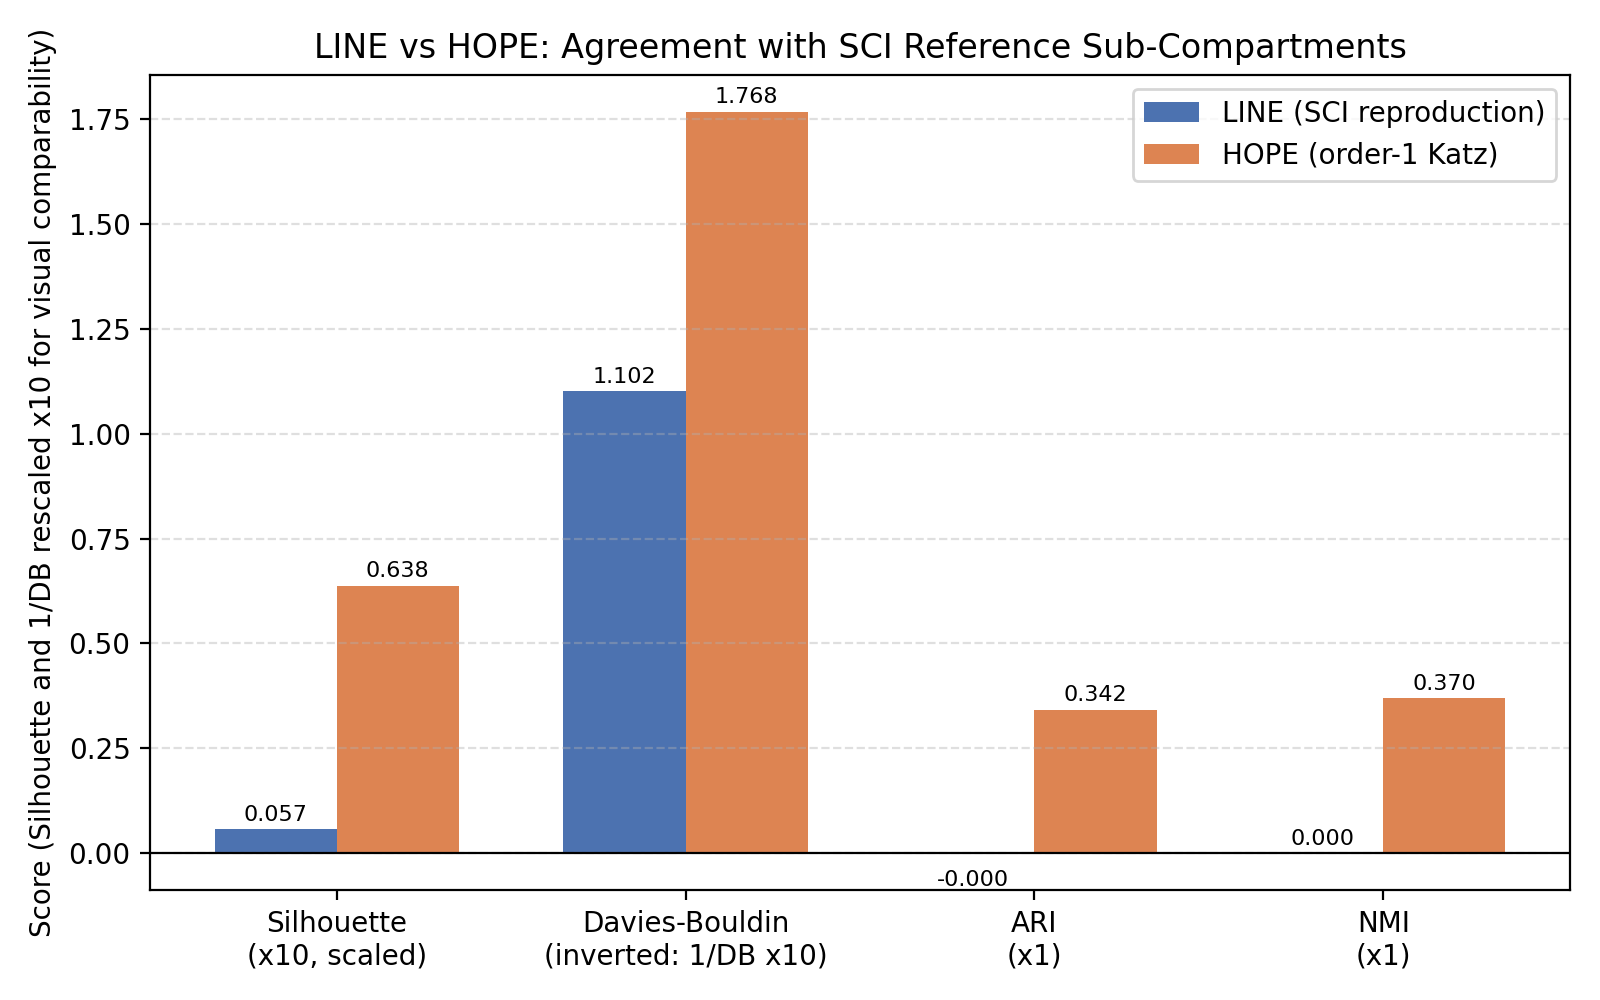
\includegraphics[width=0.32\textwidth]{comparison_chart.png}
    \vspace{-0.3cm}
    \caption{\small Comparison of clustering-quality and reference-agreement metrics for the
    reproduced LINE embedding versus the HOPE embedding. HOPE's order-1 Katz embedding shows
    markedly higher agreement with the SCI reference sub-compartment labels on every metric.}
    \label{fig:chart}
\end{figure}
\vspace{-0.8cm}

\subsection{Discussion}
On this reproduction, the HOPE embedding clusters substantially better recover the SCI reference
sub-compartment structure than the reproduced LINE embedding: an Adjusted Rand Index of
0.342 versus essentially zero, and a Normalized Mutual Information of 0.370 versus 0.00017.
The internal clustering-quality metrics tell the same story — HOPE's clusters are both more
compact (higher Silhouette Score) and better separated (lower Davies-Bouldin Index) than the
LINE embedding's clusters.

It is important to frame this result carefully: these numbers describe \textit{this reproduction},
not a definitive statement about LINE's ceiling performance as reported by Ashoor et al. (2020).
Under an identical Hi-C graph, clustering protocol, and evaluation pipeline, the Katz-based
higher-order proximity captured by HOPE's order-1 term aligned considerably more closely with
the biologically validated SCI sub-compartment calls than this project's LINE reproduction did.


% ---------------------------------------------------------------
% 7. CHALLENGES
% ---------------------------------------------------------------
\section{Challenges and Strategic Optimizations}

\subsection{Scaling the Katz Similarity Matrix}
The most significant computational obstacle encountered was scaling the higher-order Katz
similarity matrix to a genome-wide Hi-C graph. Including the two-hop term $\beta^2 A^2$ required
squaring a sparse $26{,}977 \times 26{,}977$ adjacency matrix, which produced roughly 726 million
non-zero entries — far too dense for the subsequent truncated SVD to run in a reasonable time or
memory budget. This was resolved by restricting the HOPE similarity matrix to its order-1 term
only ($S = \beta A$), which kept the problem tractable while still capturing meaningfully more
global structure than LINE's purely local sampling, as reflected in the results above.

\subsection{Legacy Dependency Chain in sci-DNN}
The sci-DNN companion classifier was written against Python 2.7-era conventions and an older
Keras/TensorFlow API. Running it in a modern Python 3 environment required reconciling
incompatible package versions and API signatures, which was a non-trivial setup task separate
from the core graph-embedding work.

\subsection{Handling a Genome-Scale Interaction File}
The raw Hi-C interaction file is approximately 513 MB and expands into tens of millions of directed
edge entries once parsed. Building the sparse adjacency matrix directly from streamed edge
triples (row, column, weight), rather than materializing a dense matrix at any point, was necessary
to keep memory usage within the limits of the available hardware.

\subsection{Partial Overlap with the Reference Label Set}
Of the 26,977 genomic bins clustered by both embeddings, only 26,226 bins (97.2\%) had a
corresponding reference sub-compartment call in the published SCI bed file, with the remaining
751 bins falling outside the reference's covered genomic regions. All external agreement metrics
(ARI and NMI) reported in Section~6 are therefore computed strictly over this overlapping bin
set, rather than the full clustered bin set, so that the comparison between LINE and HOPE is not
confounded by bins for which no ground-truth label exists. This restriction was applied
identically to both embeddings to keep the comparison fair.


% ---------------------------------------------------------------
% 8. FUTURE WORK
% ---------------------------------------------------------------
\section{Future Work}

As the project advances beyond the mid-term review, the following directions are planned:

\begin{itemize}
    \item \textbf{Scalable Higher-Order HOPE:} Investigate sparse approximation or low-rank
    truncation strategies that would allow the two-hop (and higher) Katz terms to be included in
    the HOPE similarity matrix without the 726-million-entry blow-up encountered in this phase,
    to test whether capturing even more global structure further improves agreement with the
    SCI reference.

    \item \textbf{Three-Way Comparison with sci-DNN:} Incorporate the predicted labels from the
    sci-DNN classifier as a third point of comparison alongside the LINE and HOPE embeddings,
    evaluating all three under the same ARI/NMI framework against the SCI reference.

    \item \textbf{Cross-Cell-Line Validation:} Extend the comparison beyond GM12878 to additional
    Hi-C datasets from other cell lines, to assess whether HOPE's advantage over LINE observed in
    this reproduction generalizes or is specific to this dataset.

    \item \textbf{LINE Hyperparameter Sensitivity:} Systematically vary LINE's embedding
    dimensionality, number of negative samples, and training-sample budget to determine whether
    the reproduced LINE embedding's low agreement with the SCI reference is an artifact of this
    reproduction's specific hyperparameter choices rather than a ceiling on LINE's performance.

    \item \textbf{Orthogonal Validation:} Incorporate independent ChIA-PET interaction data, as
    used in the original SCI paper, to validate both the LINE and HOPE sub-compartment calls
    against a biological signal that is independent of the Hi-C contact graph itself.

    \item \textbf{Runtime and Memory Benchmarking:} Quantify and compare the wall-clock time and
    peak memory footprint of the LINE and HOPE embedding pipelines on the same hardware, to
    characterize the practical scalability trade-off between the two methods alongside their
    accuracy trade-off.
\end{itemize}


% ---------------------------------------------------------------
% 9. CONCLUSION
% ---------------------------------------------------------------
\section{Conclusion}

This mid-term phase successfully reproduced the SCI pipeline for genomic sub-compartment
prediction from Hi-C data, reconstructing the genome-wide contact graph, generating LINE-based
embeddings, and clustering them into sub-compartments comparable to the published reference.
Building on this reproduction, an alternative graph embedding method, HOPE, was implemented
using order-1 Katz proximity and truncated SVD, and evaluated under an identical clustering and
scoring protocol. The comparison showed that, on this dataset and under this reproduction's
settings, HOPE's embedding aligned considerably more closely with the SCI reference
sub-compartment calls than the reproduced LINE embedding, as measured by both internal
clustering-quality metrics and external agreement metrics. The practical challenges of scaling
graph-embedding computations to a genome-wide Hi-C graph, and the strategies used to work
around them, have been documented as a foundation for the scalable higher-order extensions
planned for the remainder of this project.

In quantitative terms, this phase establishes two concrete reference points for the remainder of
the project: a reproduced LINE baseline (ARI $-0.00003$, NMI $0.00017$) and an order-1 HOPE
extension (ARI $0.342$, NMI $0.370$) against the SCI reference sub-compartment calls, both
computed under an identical 26,977-bin GM12878 Hi-C graph and identical $k=5$ K-means
clustering. These numbers should be read as a reproduction-specific comparison rather than a
general verdict on LINE versus HOPE, since the LINE embedding was trained with the hyperparameters
specified by the original SCI codebase rather than an independently tuned configuration. The
immediate next steps are to extend the Katz similarity matrix to its higher-order terms within a
tractable memory budget, incorporate sci-DNN as a third comparison point, and test whether the
pattern observed here generalizes beyond GM12878, as outlined in Section~8.

Beyond the specific numbers, this phase demonstrates that a full genomic sub-compartment
prediction pipeline, from a raw Hi-C interaction file through graph construction, embedding,
clustering, and external biological validation, can be reproduced and meaningfully extended
within the computational constraints of a course project, provided the engineering trade-offs
documented in Section~7 are addressed deliberately rather than avoided.
The order-1 Katz restriction adopted for HOPE is one such trade-off, and the fact that it still
outperformed the reproduced LINE baseline on every metric suggests that, for this dataset, even
a computationally cheap higher-order proximity measure carries more genuine sub-compartment
signal than the purely local embedding LINE produced here.


% ---------------------------------------------------------------
% 10. APPENDIX
% ---------------------------------------------------------------
\section{Appendix}

\subsection*{A.1 Full Evaluation Output}
Table~\ref{tab:appendix} reproduces the complete, unrounded metric output recorded in the
evaluation metrics file (\texttt{results/evaluation\_metrics.txt}) for both embeddings evaluated
in this report.

\begin{table}[h]
\centering
\small
\caption{Full evaluation output for the LINE and HOPE embeddings.}
\label{tab:appendix}
\begin{tabular}{lcc}
\toprule
\textbf{Metric} & \textbf{LINE (order 1+2)} & \textbf{HOPE (order-1 Katz)} \\
\midrule
Clustered bins (internal metrics) & 26977 & 26977 \\
Silhouette Score & 0.00569 & 0.06380 \\
Davies-Bouldin Index & 9.0750 & 5.6569 \\
Overlap bins with reference & 26226 & 26226 \\
Adjusted Rand Index (ARI) & -0.00003 & 0.34236 \\
Normalized Mutual Info (NMI) & 0.00017 & 0.36976 \\
\bottomrule
\end{tabular}
\end{table}

\subsection*{A.2 Reproduction Environment and Hyperparameters}
Table~\ref{tab:env} summarizes the software environment and key hyperparameters used to
produce the results reported above, to support exact reproduction of this phase of the project.

\begin{table}[h]
\centering
\caption{Software environment and hyperparameter settings.}
\label{tab:env}
\begin{tabular}{ll}
\toprule
\textbf{Setting} & \textbf{Value} \\
\midrule
Hi-C dataset & GM12878, 26{,}977 genomic bins \\
LINE embedding dimension & 100 (order-1) + 100 (order-2), concatenated to 200 \\
HOPE embedding dimension & 100 (rank-100 truncated SVD) \\
HOPE decay factor $\beta$ & $0.5 \,/\, \text{max weighted degree of } A$ \\
K-means clusters ($k$) & 5, fixed random seed shared across LINE and HOPE \\
Evaluation metrics & Silhouette, Davies-Bouldin, ARI, NMI \\
Core libraries & Python 3, NumPy, SciPy, scikit-learn \\
\bottomrule
\end{tabular}
\end{table}

\subsection*{A.3 Repository and Output Artifacts}
The reproduction and extension described in this report are organized into three top-level
directories: \texttt{repos/} containing the cloned SCI and sci-DNN codebases, \texttt{data/}
containing the raw GM12878 Hi-C interaction file, and \texttt{results/} containing every
generated artifact referenced in this report — the constructed Hi-C graph, the LINE and HOPE
embeddings, the K-means compartment assignments for both methods, and the final evaluation
metrics file summarized in Table~2. This separation keeps the original third-party codebases
isolated from the project-specific outputs, so that the HOPE extension could be developed and
re-run independently of the upstream SCI pipeline.

% ---------------------------------------------------------------
% 11. REFERENCES
% ---------------------------------------------------------------
\section{References}

\begin{enumerate}
    \item Ashoor, H., Chen, X., Rosikiewicz, W., Wang, J., Cheng, A., Wang, P., Ruan, Y., \& Li, S.
    (2020). \textit{Graph embedding and unsupervised learning predict genomic sub-compartments
    from HiC chromatin interaction data}. Nature Communications, 11, 1173.

    \item Tang, J., Qu, M., Wang, M., Zhang, M., Yan, J., \& Mei, Q. (2015). \textit{LINE:
    Large-scale Information Network Embedding}. Proceedings of the 24th International
    Conference on World Wide Web (WWW), 1067--1077.

    \item Ou, M., Cui, P., Pei, J., Zhang, Z., \& Zhu, W. (2016). \textit{Asymmetric Transitivity
    Preserving Graph Embedding}. Proceedings of the 22nd ACM SIGKDD International
    Conference on Knowledge Discovery and Data Mining, 1105--1114.

    \item Rao, S. S. P., Huntley, M. H., Durand, N. C., et al. (2014). \textit{A 3D Map of the
    Human Genome at Kilobase Resolution Reveals Principles of Chromatin Looping}. Cell,
    159(7), 1665--1680.

    \item Pedregosa, F., Varoquaux, G., Gramfort, A., Michel, V., Thirion, B., Grisel, O., et al.
    (2011). \textit{Scikit-learn: Machine Learning in Python}. Journal of Machine Learning
    Research, 12, 2825--2830.

    \item Harris, C. R., Millman, K. J., van der Walt, S. J., Gommers, R., Virtanen, P.,
    Cournapeau, D., et al. (2020). \textit{Array Programming with NumPy}. Nature, 585,
    357--362.

    \item Virtanen, P., Gommers, R., Oliphant, T. E., Haberland, M., Reddy, T., Cournapeau, D.,
    et al. (2020). \textit{SciPy 1.0: Fundamental Algorithms for Scientific Computing in
    Python}. Nature Methods, 17, 261--272.

    \item Rousseeuw, P. J. (1987). \textit{Silhouettes: A Graphical Aid to the Interpretation
    and Validation of Cluster Analysis}. Journal of Computational and Applied Mathematics,
    20, 53--65.

    \item Davies, D. L., \& Bouldin, D. W. (1979). \textit{A Cluster Separation Measure}.
    IEEE Transactions on Pattern Analysis and Machine Intelligence, PAMI-1(2), 224--227.

    \item Hubert, L., \& Arabie, P. (1985). \textit{Comparing Partitions}. Journal of
    Classification, 2(1), 193--218.
\end{enumerate}

\end{document}
